% GENERATED FROM typst/manual/sections/02_mapping_error.typ BY scripts/typ2tex.py (v1.0.0) — DO NOT EDIT.
% Edit canonical Typst under typst/ and regenerate with: python3 scripts/typ2tex.py --root . --outdir latex

\section{Typed maps and exact uncertainty examples}\label{manual:m3-mapping-error}

These examples instantiate \mainsection{main:sec:m3-maps} using rational
addition, subtraction, multiplication and division.
They follow \secref{manual:calculation-spine}: declare the inputs and map,
compute exact outputs, and compare under a stated joint uncertainty model.
The examples below are conditional calculations; the published-input example
retains its measurement provenance.

\paragraph{Mapping records and composition.}
Inputs and outputs retain quantity kind, dimension, unit, admissible bounds, scope and
lineage. Dimensions use the declared ordered basis length, time and count.
Native counts, cycle counts and dimensionless report coordinates remain distinct
through kind and unit checks. Every parameter binds a source identity, payload
key, exact value, dimension and origin. Raw inputs bind their values to trusted
source payloads; intermediate values carry a reproducible upstream execution.
Map versions, code, specifications, inputs and source payloads receive separate
hashes.

The worked composition takes $x=3$, $f(x)=2x$, and $g(y)=2y$.
Its output is $12$. Both stages retain the same factor-source identity;
the source appears once in the composed dependency set. The complete first
codomain must lie inside the second domain. Mismatched dimensions, units,
scopes and lineages reject composition. Evaluation-role sources reject both
direct use in a prediction and indirect use through upstream provenance.
Fitted parameters require declared calibration exposure and an applicable
calibration budget component.

\paragraph{Exact projection and information loss.}
The map $P(x,h)=x$ maps $(3,0)$ and $(3,1)$ to the same scalar.
Both original input records remain in the execution provenance. Its arithmetic
error is zero; recovering $h$ from the projected scalar is nonunique.
No scalar reconstruction error is assigned without a declared task metric.
Affine injectivity is checked by exact matrix rank.
Unproved nonlinear injectivity remains unknown.

\paragraph{Joint laws and linearized diagnostics.}
The probabilities in these finite examples are declared model inputs.
For each stated finite joint law the implementation enumerates all atoms and
computes the exact mean and variance of
\mainequation{main:eq:m3-finite-law}. It also reports the distinct first-order
quantity in \mainequation{main:eq:m3-linear-covariance}. Covariance validation
uses exact rational Schur complements and retains singular positive-semidefinite
matrices. Missing covariance is not replaced by zero. A supplied covariance
matrix that disagrees with the supplied joint law is rejected.

Two finite examples use
$\Pr(\delta=-1/100)=\Pr(\delta=1/100)=1/4$ and
$\Pr(\delta=0)=1/2$. The dimensionless interval model is
$T=1/[(1+\delta)(1-\delta)]$. Its first-order variance is zero, but

\[
\mathbb{E}[T]=\frac{19999}{19998},\qquad\operatorname{Var}(T)=\frac{1}{399920004}>0.
\]

The near-cancelled product is
$F=(1+\delta)(1-999\delta/1000)$. Its exact results are

\[
\mathbb{E}[F]=\frac{19999001}{20000000},\qquad\operatorname{Var}(F)=\frac{1018001}{400000000000000},\qquad J\Sigma J^{\mathsf{T}}=\frac{1}{20000000000}.
\]

The full variance is more than forty times the nonzero linearized diagnostic.
The exact mean shift is $-999/20000000$. Small marginal uncertainties
therefore do not certify the omitted nonlinear contribution.

A further example uses
$R=1+\delta$, $f=1-\delta$, with probabilities $(1/4,1/2,1/4)$
at $\delta=(-1/2,0,1/2)$. It reproduces
$\mathbb{E}[Rf]=7/8$, $\operatorname{Var}(Rf)=1/64$, and zero
first-order variance.

\paragraph{Original reciprocal and near-cancelled laws.}
For the original interval example, let $y=d/s=\pm a$ with equal
probabilities, $a=1/1000$, and $U=T/s=1/(1+y)+y$. Direct enumeration gives

\begin{equation}\label{eq:manual-m3-original-interval}
\mathbb{E}[U]=\frac{1}{1-a^2}=\frac{1000000}{999999},\qquad\operatorname{Var}(U)=\frac{a^6}{(1-a^2)^2}=\frac{1}{999998000001000000}.
\end{equation}

Its linearized variance is zero because the two input corrections are
the same random variable.
For the original product, let $x=(-\epsilon,0,\epsilon)$ have probabilities
$(1/4,1/2,1/4)$, with $\epsilon=1/1000$, $\delta=1/1000000$,
$b=1-\delta$, and $V=F/\mathrm{Hz}=(1+x)(1-bx)$. Then

\begin{equation}\label{eq:manual-m3-original-product}
\mathbb{E}[V]=1-\frac{b\epsilon^2}{2},\qquad\operatorname{Var}(V)=\frac{\delta^2\epsilon^2}{2}+\frac{b^2\epsilon^4}{4}.
\end{equation}

The first term is the linearized variance; the full variance is
$500000.0000005$ times as large. These joint laws retain the input
dependence. They are distinct from the three controls above.
The authenticated original probe and its unchanged failing historical
implementation are retained with their source and output bindings.
The successor computes exact finite-law moments; covariance alone still
leaves nonlinear output moments unresolved.

\paragraph{Legitimate cancellation and limits of moments.}
Let $X$ take $-\epsilon,0,\epsilon$ with probabilities
$1/4,1/2,1/4$, $\epsilon>0$. For $h(X)=X^2$, the linearized
variance at zero vanishes, but the exact mean and variance are
$\epsilon^2/2$ and $\epsilon^4/4$. Treating the zero derivative as a
proof of zero spread contradicts \mainequation{main:eq:m3-finite-law}.

A shared offset cancels in $(a+X)-(b+X)=a-b$. Replacing it by two
independent copies changes the joint law.
For an affine endpoint difference with means $(7,2)$ and covariance
$(\begin{matrix}
4 & 4 \\
4 & 4
\end{matrix})$, the mean is
$5$ and the exact variance is zero. The model $x/x$ is constant on the
stated nonzero support and also has zero variance.
For a nonlinear map supplied only with input moments, the first-order diagnostic
is retained and output uncertainty remains unresolved.
Two laws illustrate this with identical input mean zero and
variance one: mass $1/2$ at each of $-1,1$, and masses $(1/8,3/4,1/8)$
at $(-2,0,2)$. Their squared outputs have variances zero and three,
respectively. Input means and covariances do not determine nonlinear output
uncertainty.

\paragraph{Bounds, domains and source precision.}
For $g(y)=1/y$ on a positive interval with lower endpoint $a>0$,
$L_g=a^{-2}$ suffices.
The composed-bound example instantiates
\mainequation{main:eq:m3-composed-bound}. Assume uniform bounds
$b_f=1/100$ and $b_g=1/1000$, an inner image in $[1,2]$, and the
outer reciprocal law on $[1/2,3]$. The enlarged image remains in the outer
domain. Its Lipschitz constant is $4$, giving the bound $41/1000$.
As admissible intermediate values approach zero, no finite uniform bound
follows. A denominator domain containing zero returns an undefined-or-unbounded status,
with no finite symmetric interval. A discrete joint law can still be evaluated
when its actual denominator support excludes zero, even if its mean lies at an
invalid linearization point; the first-order diagnostic is then unavailable.

Each output has a separate budget with matching dimensions and units,
distinguishing arithmetic, resolution, window, model discrepancy,
calibration, propagation, solver and comparison contributions. Bounds and
standard uncertainties bind evidence to that output. Unknown and
inapplicable components carry reasons and no numerical values. A finite-law
standard uncertainty binds the declared law and its variance. The affine
moment route instead binds complete input moments. A deterministic bound
cannot be relabelled as a standard deviation. Defining
constants have zero measurement variance, while absent realization uncertainty
remains unknown. This example has no physical discrepancy model, so its physical
budget remains partial despite exact finite arithmetic.

Synthetic printed-decimal controls test units and half-last-place bounds under
nearest rounding. Printed zero requires a source convention or remains unknown.
Numerical interpretation is checked separately from raw-byte integrity.

\paragraph{Source quantities and worked routes.}\label{manual:m3-experimental-inputs}
A quantity binds its source payload, source locator, kind, dimension, unit,
domain, meaning and uncertainty category. A separately supplied trusted source
must agree with that binding. Relabelling a dimensionless input as a frequency
therefore fails even when its numerical distribution is unchanged. A conversion
is a declared map with its own source and uncertainty. An aggregate and its
components cannot both contribute to the same budget.

The reusable record retains the original inputs, operator, intermediate
moments or intervals, exact outputs and reporting convention. For a declared
input with mean zero and variance $2$, affine propagation returns those
moments exactly. Two uses of this same input give variance zero for their
difference and $8$ for their sum. With output laws $2X\,\mathrm{Hz}$
and $3X\,\mathrm{s}$, the variances are $8\,\mathrm{Hz}^2$ and
$18\,\mathrm{s}^2$, with covariance $12\,\mathrm{Hz}\,\mathrm{s}$.
The coefficients and output types are declared conversion parameters.
For $X\in[1,3]$, reciprocal interval evaluation returns $[1/3,1]$;
an interval containing zero cannot give a finite reciprocal enclosure.
The nonlinear moment-only route retains its diagnostic and leaves the
uncomputed output moments unresolved. Variances remain rational; a square root
need not be rounded into a claimed exact standard uncertainty.

The published hydrogen example uses the corrected Table~VI value and keeps
the reference and wall corrections already included in its input. Its quoted
uncertainty remains a source report: it supplies neither missing raw campaign
data nor a joint law. Correction execution and passive comparison assessment
remain separate. The paper's mean $1420405751.768\,\mathrm{Hz}$ and
one-sigma uncertainty $0.002\,\mathrm{Hz}$~\cite{hellwig-hydrogen-1970} also give a single-quantity
moment example: treating the reported value as its mean, the identity map
retains variance $1/250000\,\mathrm{Hz}^2$. This aggregate propagation
does not reconstruct component covariance or a probability distribution.
These routes and the reduction controls are reproduced by
\texttt{python3} \texttt{manual/scripts/aod\_experimental\_comparison.py} \texttt{--check}
from \texttt{manual/data/experimental\_comparison/experimental\_input\_comparison.json}.

\paragraph{Execution and falsification.}
Run \texttt{python3 manual/scripts/aod\_mapping\_error.py --check} to
reconstruct \texttt{manual/data/mapping\_error/mapping\_error.json}.
The tests mutate source payloads, input values,
upstream execution digests, parameter origins, dimensions, domain bounds,
projection claims, covariance, missing error components and purported physical
completion. Each mutation executes the affected validator. The same guards
remain active with Python optimization enabled.

\subsection{Five-boundary provenance DAG and exact joint-law variance ledger}\label{manual:m3-maps:dec-joint-laws}

Declare the typed-map boundary stack separating source ancestry, map composition, joint-law pushforward, evaluation-role scope, and quarantined external reporting:

\[
B_{\mathrm{src}}\to B_{\mathrm{map}}\to B_{\mathrm{joint}}\to B_{\mathrm{role}}\to B_{\mathrm{ext}}.
\]

Vector \texttt{RC-036} (\texttt{manual/data/boundary\_sadar/typed\_map\_joint\_law\_ledger.csv}, verified by \texttt{python3 -B -m manual.engine} \texttt{--sector} \texttt{boundary\_sadar} and \texttt{aod-core} \texttt{--verify-vectors} \texttt{--check-zero-float}) evaluates exact rational means, exact pushforward variances, and naive first-order linearized variances across all five nonlinear/shared-disturbance fixtures while deduplicating diamond provenance ($x=3\to6\to12$ retains one unique source rather than two independent copies) and enforcing disjoint calibration, validation, and held-out boundary scopes.

\begin{figure}[H]
\centering
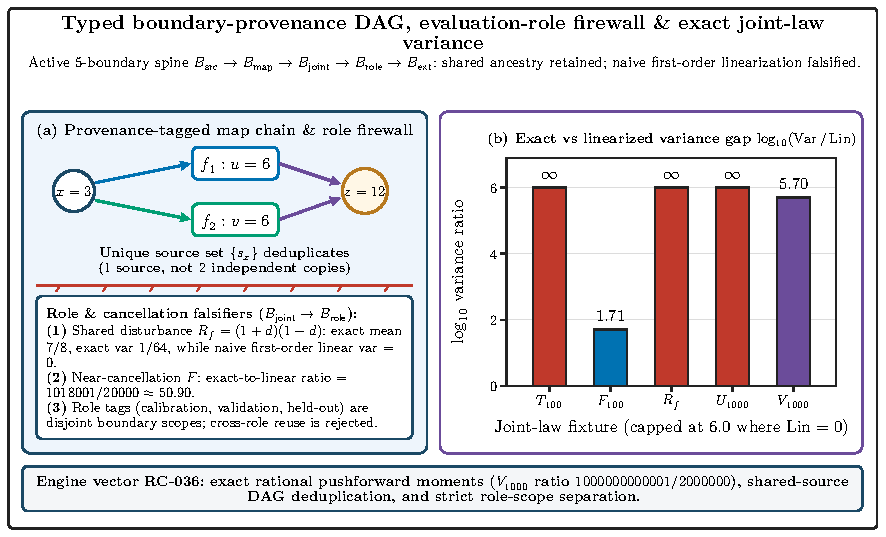
\includegraphics[width=0.92\linewidth,height=0.78\textheight,keepaspectratio]{figures/generated/typed-map-variance-feynman.pdf}
\caption{Typed boundary-provenance DAG, evaluation-role firewall, and exact versus linearized variance ratios across all five joint-law fixtures (\texttt{typed\_map\_joint\_law\_ledger.csv}).}
\label{fig:manual-typed-map-variance-feynman}
\end{figure}

\begin{table}[H]
\centering
\caption{Exact rational pushforward moments versus naive first-order linearization across typed-map joint laws (\texttt{RC-036}).}
\label{tab:manual-typed-map-joint-laws}
{\footnotesize
\begin{tabular}{llrrrr}
\toprule
Law ID & Map formula & Exact mean & Exact variance & Linear var & Exact / linear \\
\midrule
\texttt{T\_interval\_100} & $1/\left[(1+d)(1-d)\right]$ & $19999/19998$ & $1/399920004$ & $0/1$ & div-by-zero ($\operatorname{Lin}=0$) \\
\texttt{F\_near\_cancel\_100} & $(1+d)(1-999d/1000)$ & $19999001/20000000$ & $1018001/(4\cdot10^{14})$ & $1/(2\cdot10^{10})$ & $1018001/20000$ \\
\texttt{Rf\_symmetric\_2} & $(1+d)(1-d)$ & $7/8$ & $1/64$ & $0/1$ & div-by-zero ($\operatorname{Lin}=0$) \\
\texttt{U\_orig\_recip\_1000} & $1/(1+y)+y$ & $1000000/999999$ & $1/999998000001000000$ & $0/1$ & div-by-zero ($\operatorname{Lin}=0$) \\
\texttt{V\_orig\_prod\_1000} & $(1+x)(1-bx)$ & $1999999000001/(2\cdot10^{12})$ & $1000000000001/(4\cdot10^{24})$ & $1/(2\cdot10^{18})$ & $1000000000001/2000000$ \\
\bottomrule
\end{tabular}
}
\end{table}
